\documentclass{scrartcl}
\usepackage[dvipsnames]{xcolor}
\usepackage{tikz,color}
\usetikzlibrary{arrows,automata,positioning}
\newcommand{\overbar}[1]{\mkern 1.5mu\overline{\mkern-1.5mu#1\mkern-1.5mu}\mkern 1.5mu}
\oddsidemargin=-1in
\evensidemargin=-1in
\topmargin=-2in
\begin{document}
\begin{figure}
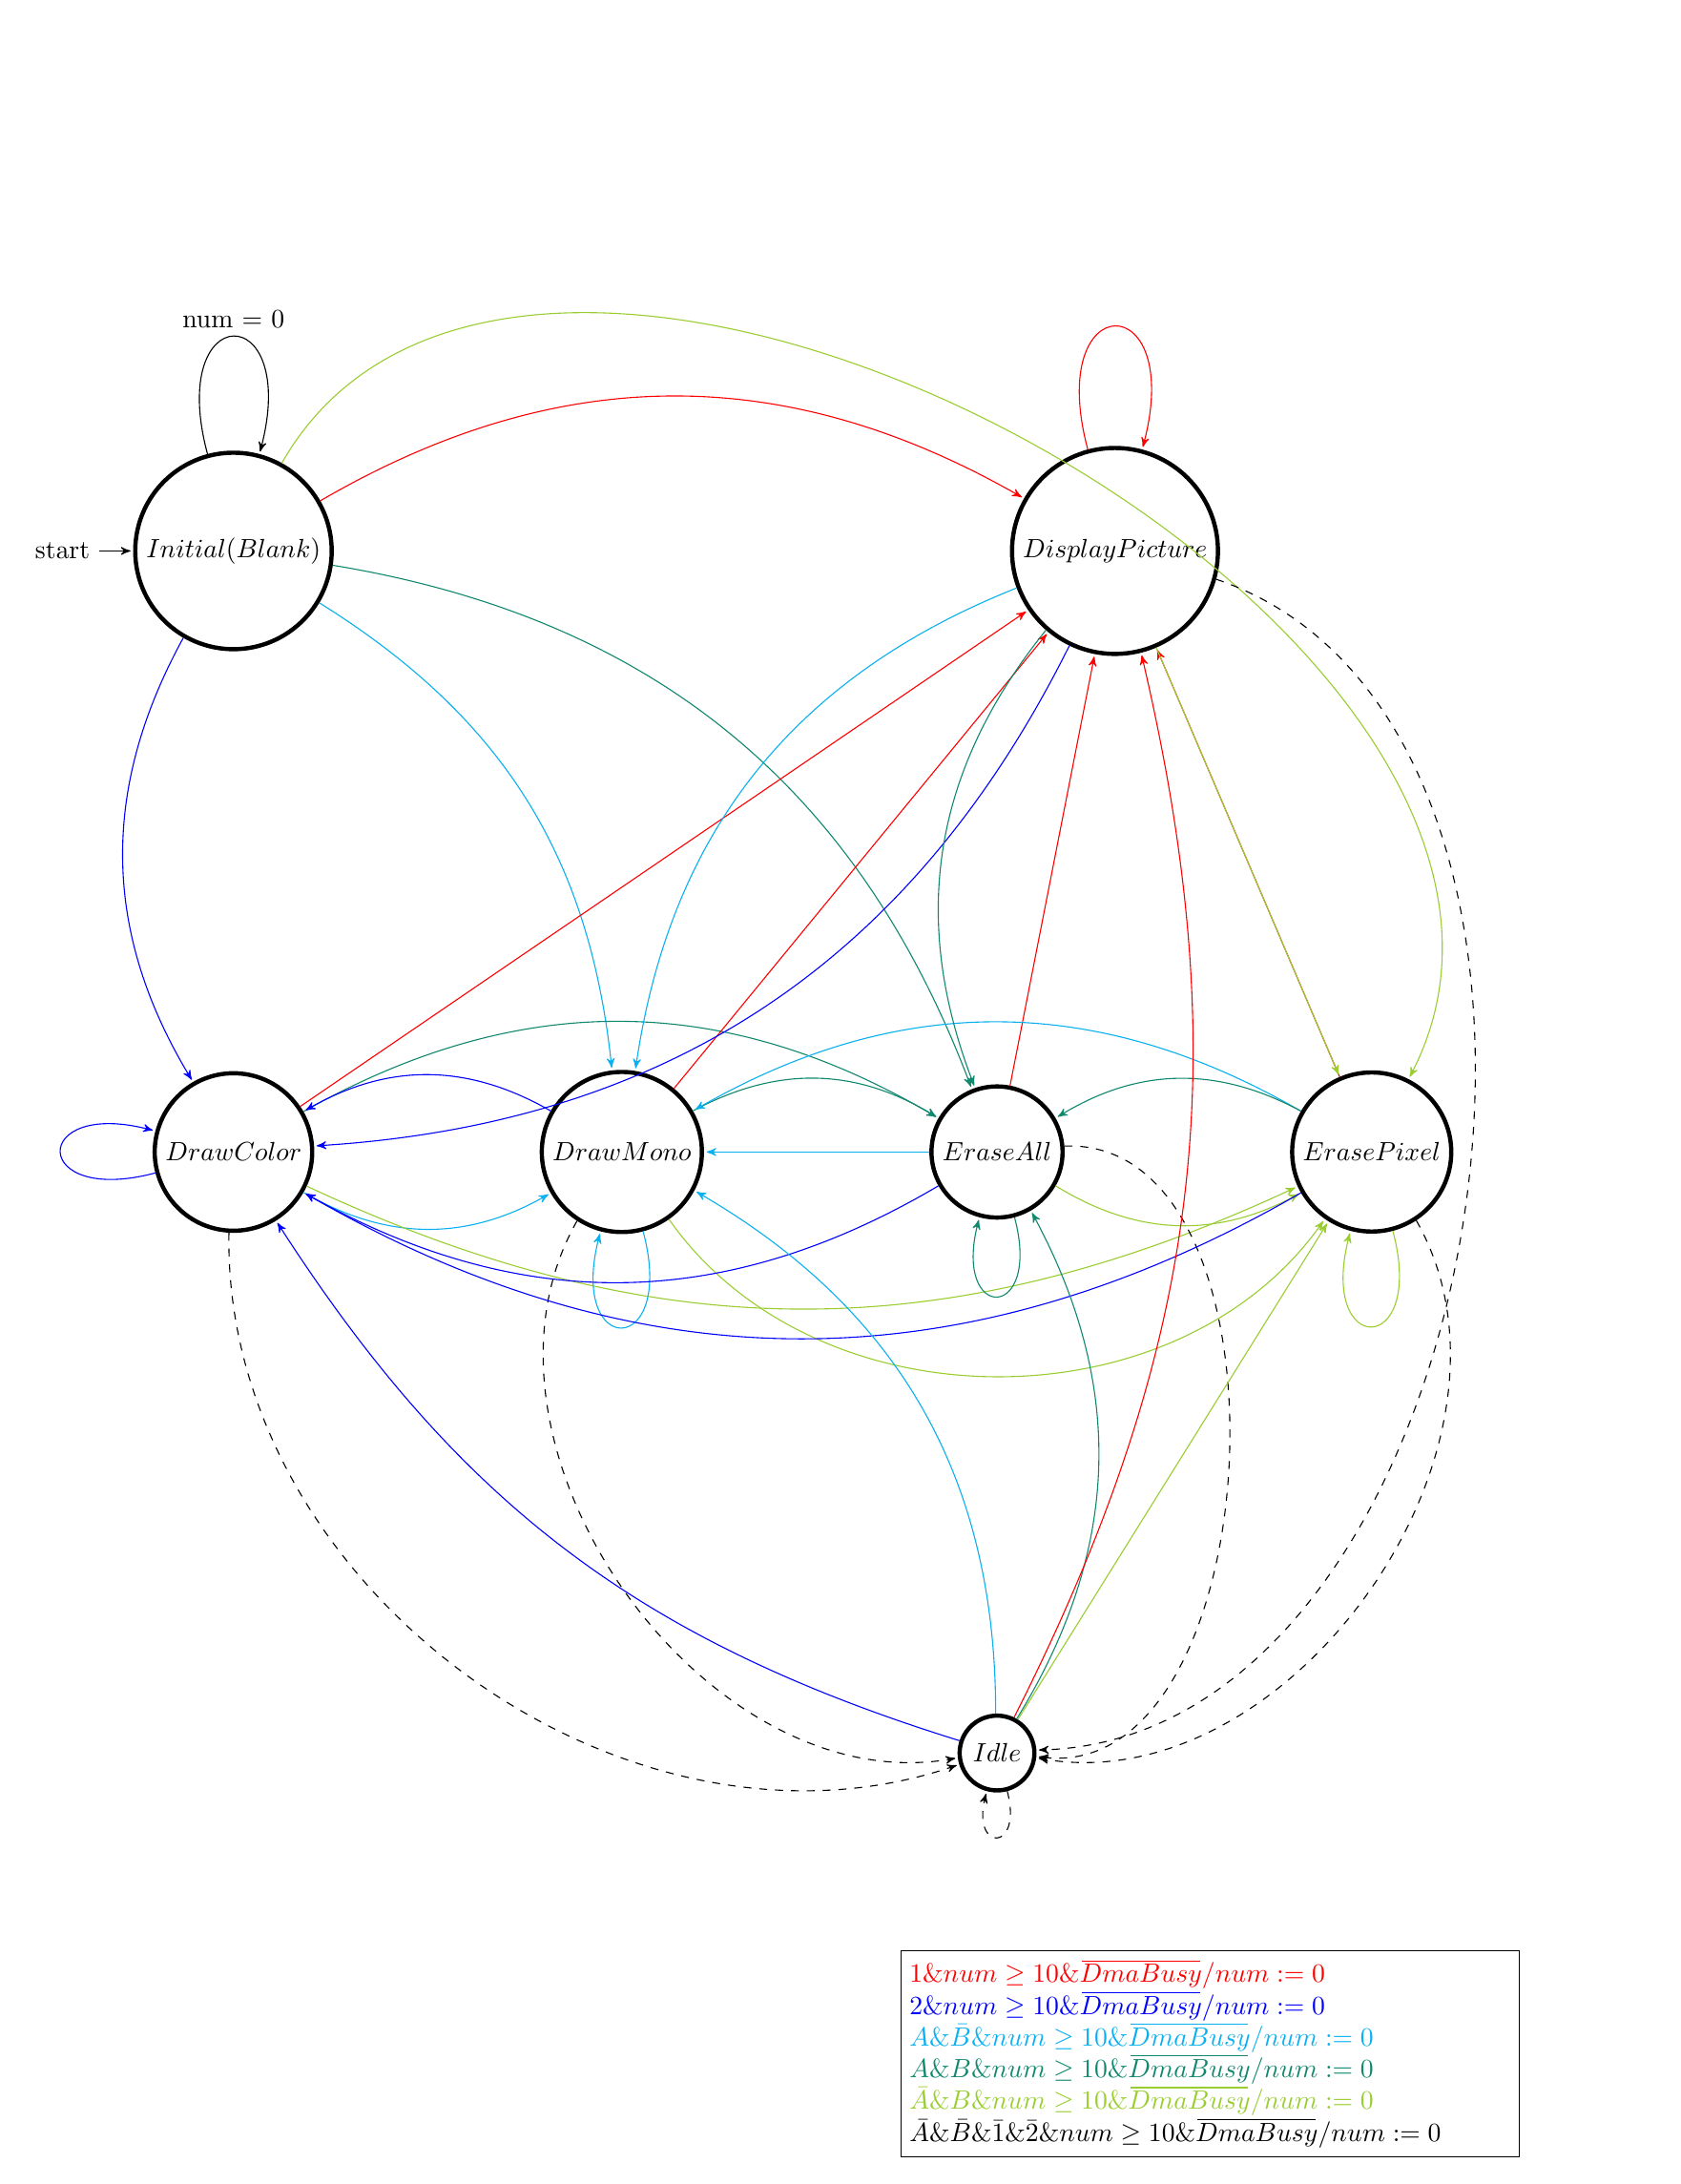
\begin{tikzpicture}[>=stealth',shorten >=1pt,auto,node distance=8cm]
  \node[initial,state] (S)    [ultra thick]  {$Initial (Blank)$};
  \node[state]         (s1) [below of=S,ultra thick]  {$Draw Color$};
  \node[state]         (s2) [right =3cm of s1,ultra thick] {$Draw Mono$};
  \node[state]         (s3) [right =3cm of s2,ultra thick] {$Erase All$};
  \node[state]         (s4) [right =3cm of s3,ultra thick] {$Erase Pixel$};
  \node[state]         (s5) [right =9cm of S,ultra thick] {$Display Picture$};
  \node[state]         (s6) [below of=s3,ultra thick] {$Idle$};


  \path[->] (S)  edge [loop above] node {num = 0} (S)
             edge   [bend right,blue]           node {} (s1)
             edge   [bend left=26,ProcessBlue]         node {} (s2)
             edge   [bend left= 30,PineGreen]           node {} (s3)
             edge   [bend left=89,YellowGreen]           node {} (s4)
             edge   [bend left,red]           node {} (s5)
        (s1) edge [loop left, blue]  node {} (s1)
             edge [bend right,ProcessBlue]             node {} (s2)
             edge [bend left,PineGreen]             node {} (s3)
             edge [bend right = 25,YellowGreen]             node {} (s4)
             edge  [red]            node {} (s5)
             edge [bend right = 55,dashed] node {} (s6)
        (s2)  edge [loop below,ProcessBlue]  node {}  (s2)
        	 edge  [bend right,blue]            node {} (s1)
             edge [bend left,PineGreen]             node {} (s3)
             edge [bend right= 55,YellowGreen]             node {} (s4)
             edge [red]             node {} (s5)
             edge [bend right = 65,dashed] node {} (s6)
         (s3)  edge  [ProcessBlue]                     node {}  (s2)
        	 edge  [bend left,blue]            node {} (s1)
             edge  [loop below,PineGreen]                       node {} (s3)
             edge [bend right,YellowGreen]             node {} (s4)
             edge [red]             node {} (s5)
             edge [bend left = 95,dashed] node {} (s6)
         (s4)  edge  [bend right, ProcessBlue]                     node {}  (s2)
        	 edge  [bend left,blue]            node {} (s1)
             edge  [bend right,PineGreen]                       node {} (s3)
             edge [loop below,YellowGreen]             node {} (s4)
             edge   [red]           node {} (s5)
             edge [bend left = 65,dashed] node {} (s6)
         (s5)  edge  [bend right, ProcessBlue]                     node {}  (s2)
        	 edge  [bend left,blue]            node {} (s1)
             edge  [bend right,PineGreen]                       node {} (s3)
             edge [YellowGreen]             node {} (s4)
             edge   [loop above,red]           node {} (s5)
             edge [bend right =-80,dashed] node {} (s6)
         (s6)  edge  [bend right,ProcessBlue]                     node {}  (s2)
        	 edge  [bend right = -20,blue]            node {} (s1)
             edge  [bend right,PineGreen]                       node {} (s3)
             edge [YellowGreen]             node {} (s4)
             edge   [bend right = 20, red]           node {} (s5)
             edge [loop below,dashed] node {} (s6)
          ;
\node[draw,text width=8cm] at (13,-20) { 
{\color{red} $1\&num\geq 10\& \overbar{DmaBusy}/num:=0$}\\
{\color{blue} $2\&num\geq 10\& \overbar{DmaBusy}/num:=0$}\\
{\color{ProcessBlue}$A\&\bar{B}\&num\geq 10\&\overbar{DmaBusy}/num:=0$}\\
{\color{PineGreen}$A\&B\&num\geq 10\&\overbar{DmaBusy}/num:=0$}\\
{\color{YellowGreen}\textbf{$\bar{A}\&B\&num\geq 10\&\overbar{DmaBusy}/num:=0$}}\\
{$\bar{A}\&\bar{B}\&\bar{1}\&\bar{2}\&num\geq 10\&\overbar{DmaBusy}/num:=0$}\\
};
\end{tikzpicture}
\caption{Wiisel - Finite State Machine}
\end{figure}
\end{document}